\documentclass{article}

\usepackage{graphicx}
\usepackage{float}
\usepackage{cite}
\usepackage{url}
\usepackage{caption}
\usepackage{subcaption}

\begin{document}

\section{Basic Camera Model}

The basic camera model is implemented inside the camera class. The camera class
allows the creation of rays for a given pixel. The class first uses the Up and
Lookat vectors to create an orthogonal basis w, u, v. An field of view is defined
and then used along with the value for the width, hight and current pixel location
to calculate the point on the camera screen that corresponds to the top left corner
of the pixel. Once we have the point on the screen the viewing ray can be calculated
and returned.\\

In order to create a ray given the x and y pixel locations on the output image
the angle between the x and y axis that the ray leaves the camera position are
calculated. Using these angles and the focal length of the camera the location
the ray passes through the camera plane is found and this point is used to
computed the viewing rays direction.\\

In order to implement basic anti-aliasing for each pixel 16 rays, these are aranged in
a regular grid across the pixel where each ray is 0.25 pixel widths from the previous.
The colour values for each of these rays are then averaged to give the anti-aliased
value. Figure \ref{fig:antialias} shows a raytraced sphere with and without anti-aliasing
turned on.\\

\begin{figure}[H]
  \begin{center}
  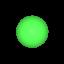
\includegraphics[width=150px]{Images/antialiasOff.png}
  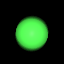
\includegraphics[width=150px]{Images/antialiasOn.png}
  \caption{Sphere raytraced with and without anti-aliasing}
  \label{fig:antialias}
  \end{center}
\end{figure}

\section{Plane \& Triangle Intersection}

The triangle intersection is done in the triangle class. The class takes three
vertexs as parameters, these are the three corners of the triangle. This first step in the
intersection test is to calculate the three vectors which make up the sides
of the triangle, these are used to get the normal by the application of the
cross product \cite{triabgle}. Using the normal and a point the intersection between the
ray and the plane the triangle lies on can be calculated then the value of t that
the ray intersects at can be found. After this the cross product is used to check
the intersection point is on the inside of each of the sides of the triangle.

\begin{figure}[H]
  \begin{center}
  
\includegraphics[width=150px]{Images/triangle.png}
  \caption{Triangle intersection}
  \label{fig:triint}
  \end{center}
\end{figure}

\section{Quadratic Intersection}

Quadratic surfaces are defined by 9 terms A - J in the equation below.

\begin{center}
$Ax^2 + 2Bxy + 2Cxz + 2Dx + Ey^2 + 2Fyz + 2Gy + Hz^2 + Iz + J = 0$
\end{center}

In order to calculate the intersection point between a ray and the surface the
ray equation $Dt + P = 0$ can be substituted into the quadratic. This substitution gives the
quadratic equation below where dx, dy and dz are the x,y and z components of the
direction and px, py and pz are the components of the initial ray position \cite{quadratic}.

\begin{center}
$Aqt^2 + Bqt + Cq = 0$ Where
$Aq = Adx^2 + Edy^2 + Hdz^2 + Bdxdy + Cdxdz + Fdydz$
$Bq = 2Apxdx + 2Epydy + 2Hpzdz + B(pxdy + pydx) + C(pxdz + pzdx) + F(pydz + pzdy) + Ddx + Gdy + Idz$
$Cq = Apx^2 + Epy^2 + Hpz^2 + Bpxpy + Cpxpz + Fpypz + Dpx + Gpy + Ipz + J$
\end{center}

This can then be solved using the quadratic equation, if there are no solutions
then the ray does not intersect the quadratic surface.

\begin{figure}[H]
\centering
\begin{subfigure}{.3\textwidth}
  \centering
  
\includegraphics[width=100px]{Images/quadCylinder.png}
  \caption{Cylinder}
\end{subfigure}%
\begin{subfigure}{.3\textwidth}
  \centering
  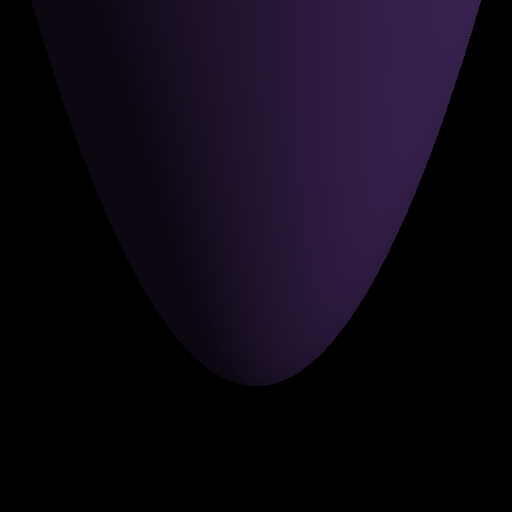
\includegraphics[width=100px]{Images/quadParaboid.png}
  \caption{Paraboid}
\end{subfigure}
\begin{subfigure}{.3\textwidth}
  \centering
  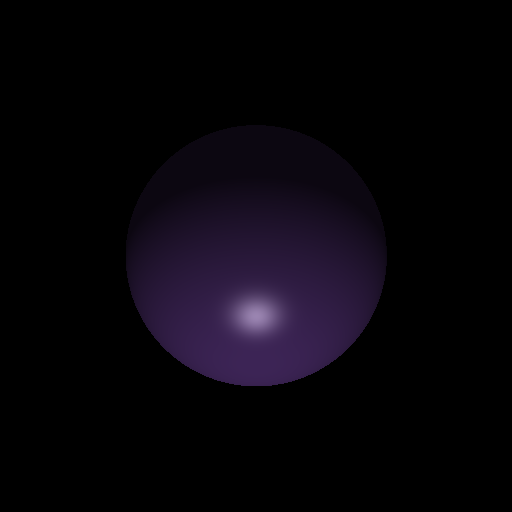
\includegraphics[width=100px]{Images/quadSphere.png}
  \caption{Sphere}
\end{subfigure}
\caption{Quadratic Surfaces}
\label{fig:quadsurface}
\end{figure}

\section{Point Lights}

Point lights are implemented in the point\_light.cpp class. The class takes a vertex
and colour as arguments as well as an optional vector for the direction of the light.
When a object is checked to get the intensity at a point if there is no direction
given the intensity of the colour given in the arguments is just returned.
When a direction has been specified the angle between the light direction and the
vector from the light to the intersection point is calculated using the dot product.
If the dot product is negative then the intensity is 0 as the angle is more than
90 degrees. Otherwise the intensity is scaled by the value of the dot product
to the power of 0.5 which is a value to control the rate of fall off.

\begin{figure}[H]
  \begin{center}
  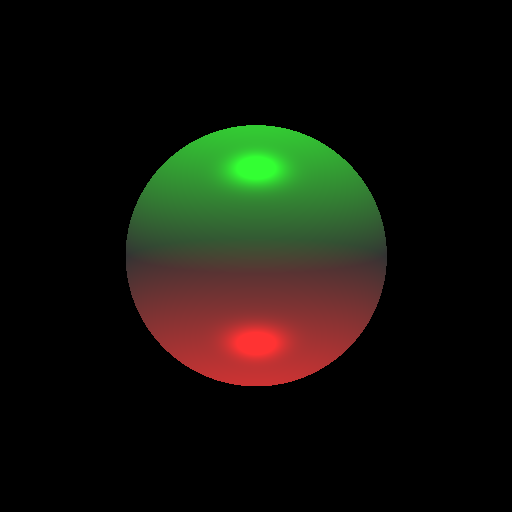
\includegraphics[width=150px]{Images/pointLight.png}
  \caption{Basic Camera Model}
  \label{fig:basiccammod}
  \end{center}
\end{figure}

\section{Specular Material}

In order to show specular materials part of the intensity at a given location is
a function of the angle between the light direction and the viewing ray direction
as defined by the Phong model. First the lights reflection ray is calculated and then
the dot product between the reflection and the viewing ray is used to scale the
specular component of the intensity.\\
The reflection ray of the viewing ray is also computed in order to calculate any
reflections in the surface. The reflection ray is ray traced in the same way as the
primary rays and the returned colour is added to the overall intensity with a
scaling value.

\begin{figure}[H]
\centering
\begin{subfigure}{.5\textwidth}
  \centering
  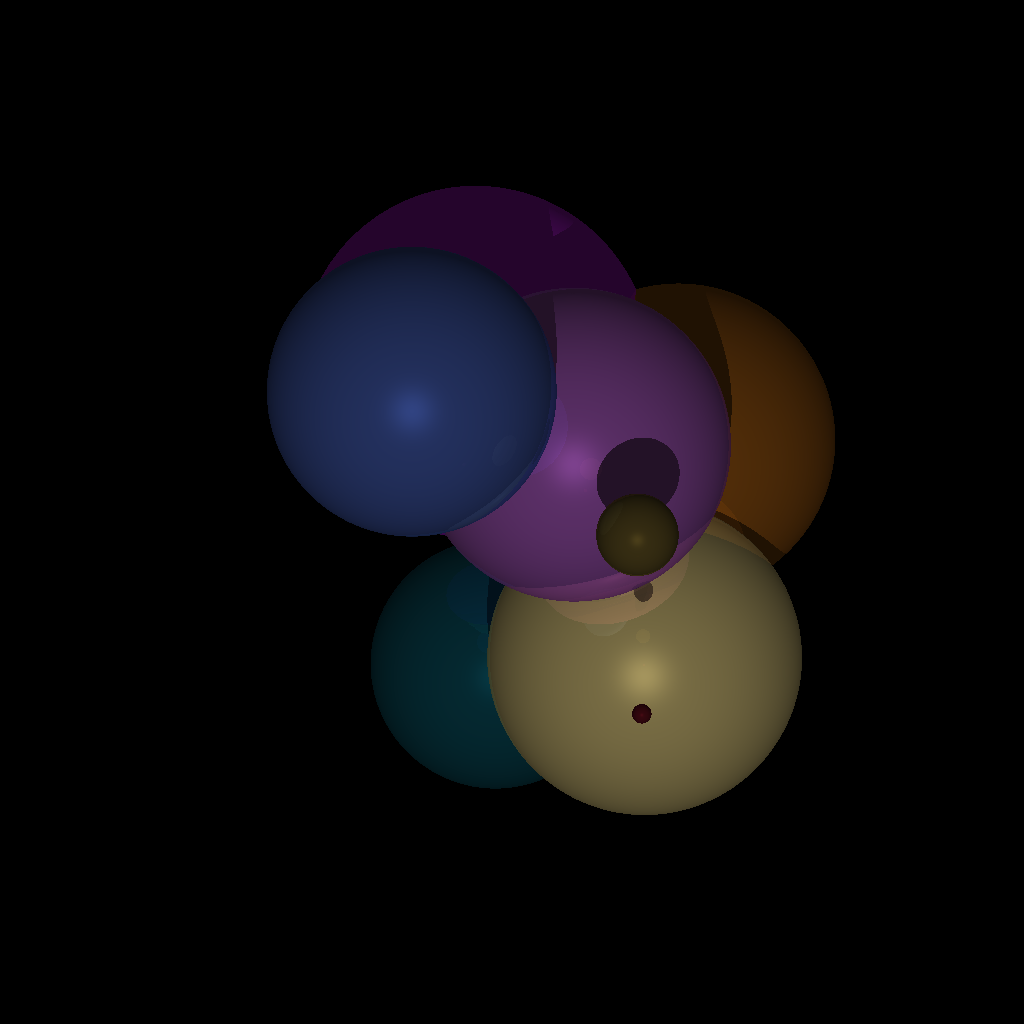
\includegraphics[width=150px]{Images/reflectionsOn.png}
  \caption{With reflection}
\end{subfigure}%
\begin{subfigure}{.5\textwidth}
  \centering
  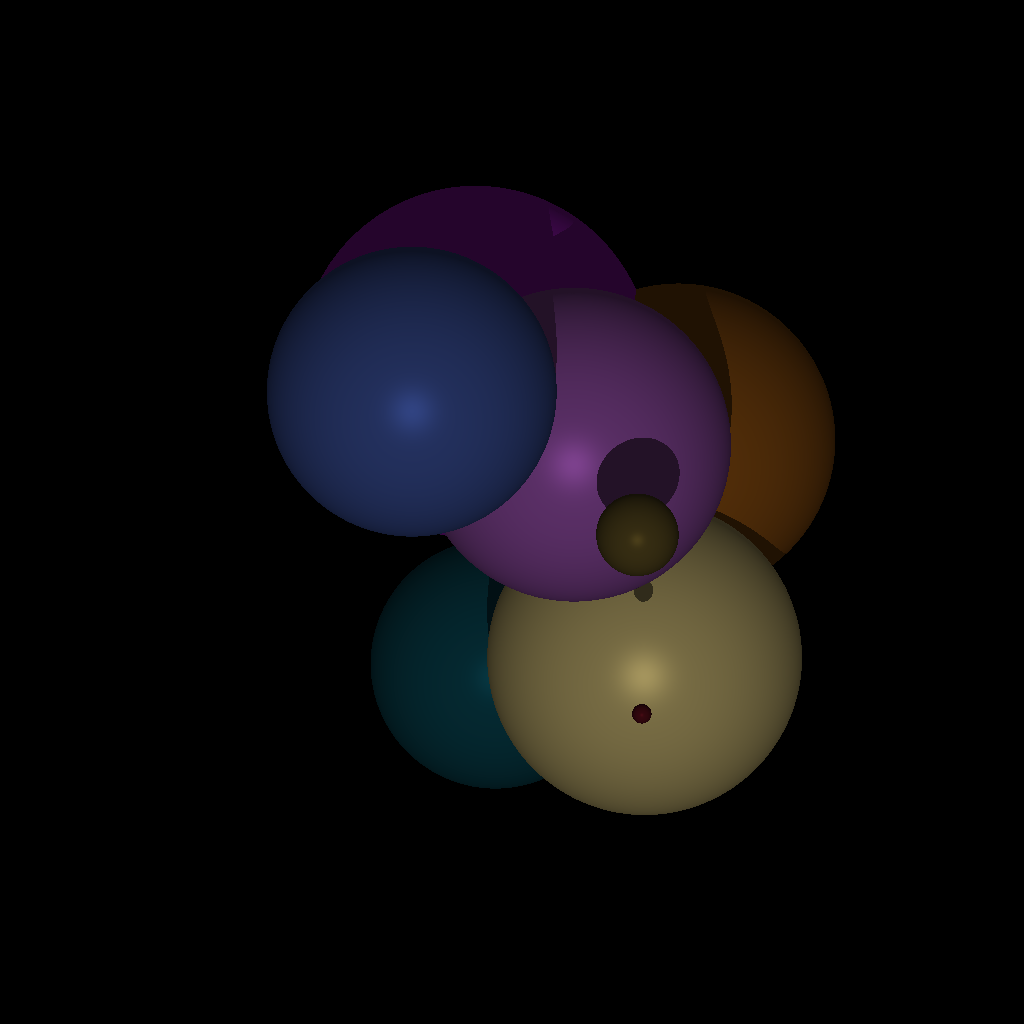
\includegraphics[width=150px]{Images/reflectionsOff.png}
  \caption{Without reflection}
\end{subfigure}
\caption{Raytraced image with and without reflection rays}
\label{fig:reflectionrays}
\end{figure}


\begin{figure}[H]
  \begin{center}
  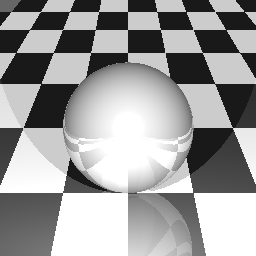
\includegraphics[width=150px]{Images/gridSphere.png}
  \caption{Basic Camera Model}
  \label{fig:basiccammod}
  \end{center}
\end{figure}

\section{Shadows}

Shadow rays are also computed at each intersection point with each of the lights.
At an intersection point the ray between the point and each of the lights is computed
and raytraced in a similar way to the primary rays, however we only care about whether
there is an intersection before the ray reaches the light. If there is an intersection
then the component of the intensity of that light is not added to the overall intensity.

\begin{figure}[H]
  \begin{center}
  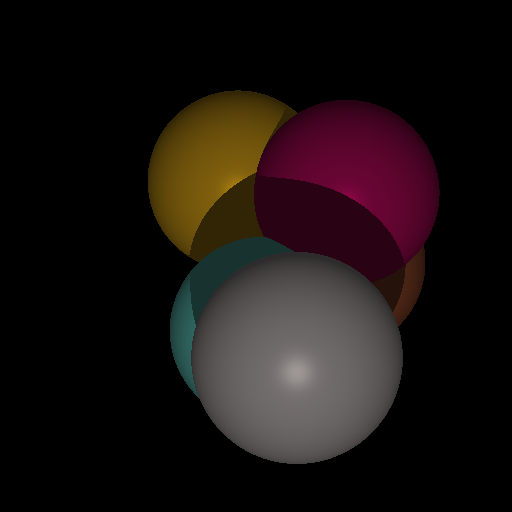
\includegraphics[width=150px]{Images/shadows.png}
  \caption{Basic Camera Model}
  \label{fig:basiccammod}
  \end{center}
\end{figure}

\section{Transparent Material}

In order to raytrace transparent materials the refracted ray must be computed at
each intersection and raytraced. The refracted ray is computed using Snells law
and then raytraced the same way as primary rays are. In order to compute the refraction
ray each object is defined a ratio of speed of light in vacuum to the speed in that
material. As the refraction ratio changes depending on whether the ray is exiting
or entering an object this needs to be computed and can be done by comparing
the dot product between the normal and the viewing ray.\\

Once the refracted ray has been raytraced the refracted component can be added
to the pixel value multiplied by a scaling value. Some transparent surfaces
can have more complex relationships between the transparent and reflective
scaling values, meaning as the angle between the normal and the viewing ray increases
the transparent component decreases and the reflective increases. In order to
compute this the Fresnel equation is used.

\begin{figure}[H]
  \begin{center}
  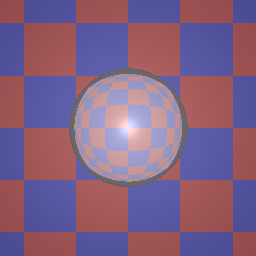
\includegraphics[width=150px]{Images/transparent.png}
  \caption{Basic Camera Model}
  \label{fig:octree}
  \end{center}
\end{figure}

\section{Octree}

In order to improve the performance of the raytracer an octree was implemented.
This consists of breaking the scene down into a set of axis aligned bounding
boxes. The boxes make up a tree with a single outer root box with eight child
boxes. The tree building algorithm is recursive firstly starting by splitting
the root box, then its children and so on until the limit of tree depth is
reached. Each time a box is added to the tree all the objects in the scene area
checked for there intersection with the box. If a box does not contain any objects
it becomes a node. Once the deptch limit is reached then all nodes have a list
of objects which are inside compiled.\\

When raytracing a ray intersections with each axis aligned bounding box is computed
and the tree is searched for node boxes that the ray passes through. When a
node box is found that the ray passes through all the objects in that box
are tested for intersections. To avoid objects which overlap bounding boxes
being tested twice each object has a property which records the last ray number
that it was tested with and if this is equal to the current ray the object is
skipped. Ray numbers are simply the result returned from the clock() function
when the ray was computed, as the clock function returns the clock ticks since
program start, this gives a unique value for each ray.\\

This improves performance significantly, the image in figure \ref{fig:octree}
is a 256 x 256 image and takes 53 seconds to compute without an octree.
With an octree enables this time is reduced to 9 second.

\begin{figure}[H]
  \begin{center}
  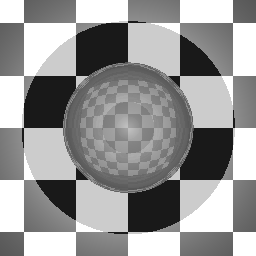
\includegraphics[width=150px]{Images/octreeTest.png}
  \caption{Basic Camera Model}
  \label{fig:octree}
  \end{center}
\end{figure}

\bibliographystyle{unsrt}
\bibliography{ref}

\end{document}